\chapter
 [Design and demonstration of an operating system for executing applications on quantum network nodes]
 {Design and demonstration of an operating system for executing applications on quantum network nodes}
\label{chp:qnodeos}

\newcommand{\CaPlus}{$^{40}$Ca$^+$}

\begin{abstract}
    The goal of future quantum networks is to enable new internet applications that are impossible to achieve using solely classical communication\cite{kimble_2008_quantum,wehner_2018_stages,vanMeter_book}.
    Up to now, demonstrations of quantum network applications\cite{barz_2012_demonstration,drmota_verifiable_2024,nadlinger_device-independent_2022} and functionalities\cite{hermans2022qubit,iuliano2024qubit,matsukevich_quantum_2009,langenfeld_quantum_2021,pfaff_unconditional_2014,chou_deterministic_2018} on quantum processors have been performed in ad-hoc software that was specific to the experimental setup, programmed to perform one single task (the application experiment) directly into low-level control devices using expertise in experimental physics.
    Here, we report on the design and implementation of the first architecture capable of executing quantum network applications on quantum processors in platform-independent high-level software.
    We demonstrate the architecture's capability to execute applications in high-level software, by implementing it as a quantum network operating system --- QNodeOS --- and executing test programs including a delegated computation from a client to a server\cite{broadbent_2009_ubqc} on two quantum network nodes based on nitrogen-vacancy (NV) centers in diamond\cite{doherty_2013,childress2013diamond}.
    We show how our architecture allows us to maximize the use of quantum network hardware, by multitasking different applications on a quantum network for the first time.
    Our architecture can be used to execute programs on any quantum processor platform corresponding to our system model, which we illustrate by demonstrating an additional driver for QNodeOS for a trapped-ion quantum network node based on a single \CaPlus atom\cite{fioretto_towards_2020}.
    Our architecture lays the groundwork for computer science research in the domain of quantum network programming, and paves the way for the development of software that can bring quantum network technology to society.
\end{abstract}

\section{Introduction}

\todo{Outline: first main result, then at the end follow sections with more details including design considerations}
The first quantum networks linking multiple quantum processors as end nodes have recently been realized as physics experiments in laboratories~\cite{moehring_2007_ion_traps,ritter_2012_elementary,hofmann_2012_heralded,stockill_2017_phasetuned,jing2019entanglement,stephenson_2020_highrate,pompili_2021_multinode,krutyanskiy_entanglement_2023} and fiber networks~\cite{liu2024creation,stolk2024metropolitan,knaut2024entanglement}, opening the tantalizing possibility of realizing advanced quantum network applications~\cite{wehner_2018_stages} such as data consistency in the cloud~\cite{benor_2005_byzantine}, privacy-enhancing proofs of deletion~\cite{poremba_quantum_2022}, exponential savings in communication~\cite{guerin_exponential_2016}, or secure quantum computing in the cloud~\cite{broadbent_2009_ubqc,childs_2005_secure_qc}. Demonstrations relied either on ad-hoc software, or chose to establish that hardware parameters were in principle good enough to support a given quantum network application, although the application itself was not realized~\cite{nadlinger_device-independent_2022,liu_2022_photonic_diqkd,zhang_2022_diqkd}.

It is a major challenge to design and implement an architecture that can enable the execution of arbitrary quantum network applications on quantum processors (\cref{qnodeos:fig:fig1}), while enabling programming in high-level software that neither depends on the underlying quantum hardware, nor requires the programmer to understand the physics of the underlying devices.  In the domain of the conventional internet, the possibility of programming arbitrary internet applications in high-level software has led to the realization of radically new communication applications by diverse communities, which had a transformative impact on our society~\cite{castells_impact_2013}. What's more, the advent of programmable hardware and new application areas sparked novel fields of computer science research and guided further hardware development.  A similar development is underway in quantum computing, where the availability of high-level programming tools allows a broad participation in developing applications~\cite{noauthor_quantum_2024}.

In realizing the first such architecture we overcome both fundamental challenges that are inherent to quantum network applications, as well as technological challenges that arise from the current state of the art of quantum network hardware.

\begin{figure}
\centering
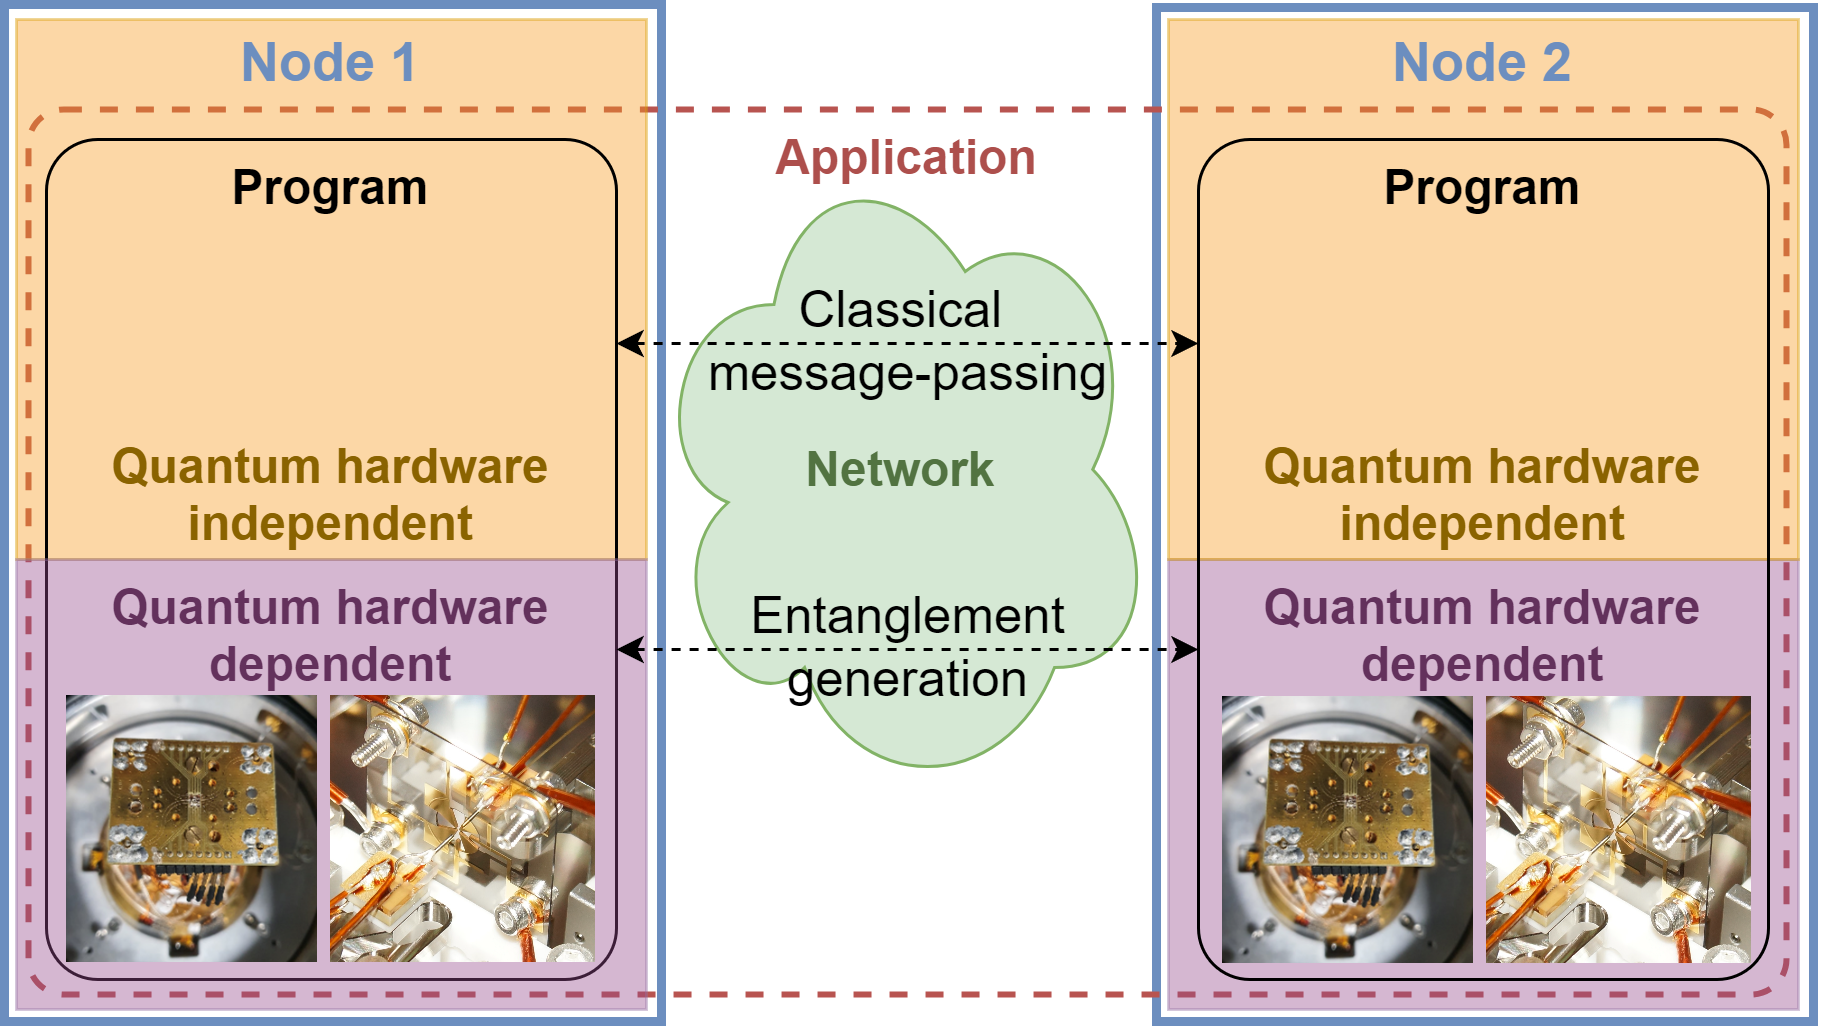
\includegraphics[width=1\linewidth]{figures/qnodeos/main/fig1/fig1.png}
\caption{\textbf{Application Paradigm.} A quantum networking application consists of multiple programs, each running on one of the end nodes~\cite{dahlberg_2022_netqasm} The distinct programs can only interact via (1) quantum communication (e.g. entanglement generation) and (2) classical communication. This allows a programmer to realize security-sensitive applications, but prohibits a global orchestration of the quantum execution, like one might do in (distributed) quantum computing~\cite{caleffi_distributed_2022} in which a single quantum program is executed on multiple nodes. Programs are written in high-level quantum hardware independent software, and executed on a quantum hardware independent system (our architecture) that controls a hardware dependent system (QDevice, \cref{qnodeos:fig:fig2}) such as a nitrogen-vacancy (NV) center node with a diamond chip (photo taken by authors, left images) or a trapped-ion quantum node~\cite{teller2023integrating} (right images). These platforms constitute physically very different QDevice systems, but can both be programmed by our architecture.}
\label{qnodeos:fig:fig1}
\end{figure}

\section{Design Considerations and Challenges}
\paragraph{Interactive Classical-Quantum Execution}
The execution of quantum network applications requires a continuing interaction between the quantum and classical parts of the execution, including interactions between different programs (\cref{qnodeos:fig:fig1}). For example, during secure quantum computing in the cloud~\cite{broadbent_2009_ubqc,ma_qenclave-practical_2022}, the program on the server is waiting for classical messages from a remote client before continuing the quantum execution at the server. This is in sharp contrast to quantum computing applications, where one quantum program can be executed in a single batch, without the need to keep quantum states live while waiting for input from other programs. In quantum computing, only relatively low-level interactions between classical and quantum processing are realized, such as in quantum error correction~\cite{lidar2013quantum}, or mid-circuit measurements~\cite{botelho_error_2022}. Higher-level classical-quantum interactions in quantum computing~\cite{bharti_noisy_2022} do not keep qubits live in memory.

We assume that the programs are divided into classical and quantum blocks of instructions (by a programmer or a compiler). Classical blocks consist of local classical operations executed on a conventional classical processor, as well as networked classical operations (i.e. sending messages to remote nodes) executed using network devices. Quantum blocks consist of local quantum operations (gates, measurements, classical control logic), as well as networked quantum operations (entanglement generation) executed on quantum hardware. A single quantum block, in essence, corresponds to a program in quantum computing, and may contain simple classical control logic, such as for the purpose of mid-circuit measurements~\cite{botelho_error_2022}.

\paragraph{Different Hardware Platforms}
Interfacing with different hardware platforms presents technological challenges: currently, a clear line between software and hardware has not been defined, and the low-level control of present-day quantum processor hardware has been built to conduct physics experiments. Early microarchitectures~\cite{bertels_quantum_2020,fu_2019_eqasm} and operating systems~\cite{giortamis_qos_2024,kong_2021_origin} for quantum computing do not address the execution of quantum network applications. We thus have to define a hardware abstraction layer (HAL), capable of interfacing with present-day quantum network setups. 

\paragraph{Timescales}
It is a fundamental challenge that different parts of such a system operate at vastly different timescales. For nodes separated by hundreds of kilometers, the duration of network operations is in the millisecond (ms) regime, and some applications~\cite{wehner_2018_stages} need  significant local classical processing (ms). In contrast, the time to execute quantum operations on processing nodes is in the regime of microseconds ($\mu$s), and the low-level control (including timing synchronization between neighboring nodes to generate entanglement~\cite{humphreys_2018_delivery}) requires nanosecond (ns) precision.

\paragraph{Memory Lifetimes}
Present-day quantum network nodes have short coherence times, posing a technological challenge to ensure operations are executed within the timeframe allowed by the quantum memory.

\paragraph{Scheduling Local and Network Operations}
In contrast to classical networking, entanglement is a form of stateful connection already at the physical layer where both nodes hold one qubit. Heralded entanglement generation requires agreement between neighboring network nodes to trigger entanglement generation in precise time-bins~\cite{dahlberg_2019_egp}, organized into a network schedule~\cite{skrzypczyk_2021_arch} that dictates when nodes make entanglement. It is a technological challenge to manage the interdependencies between the schedule of local operations, and the networked operations, since in all current processing node implementations~\cite{pompili_2021_multinode,drmota_robust_2023}, entanglement generation cannot be performed simultaneously with local operations~\cite{pompili_2021_multinode,krutyanskiy_light-matter_2019}. While interdependencies may be mitigated in the future~\cite{vardoyan_2022_netarch}, this implies that we cannot schedule (i.e. decide when to execute) the execution of local quantum operations independently of the network schedule.

\paragraph{Multitasking}
When executing quantum network applications, one node is typically idle while waiting for the other node before it can continue execution. It is hence a fundamental challenge how we can increase the utility of the system by performing multitasking~\cite{mccullough_design_1965-1,dennis_segmentation_1965}, that is, allowing the concurrent execution of several programs at once to make use of idle times. Consequently, there is a need for managing state and resources for multiple independent programs, including processes, quantum memory management, and entanglement requests. 

\begin{figure*}[htb]
\centering
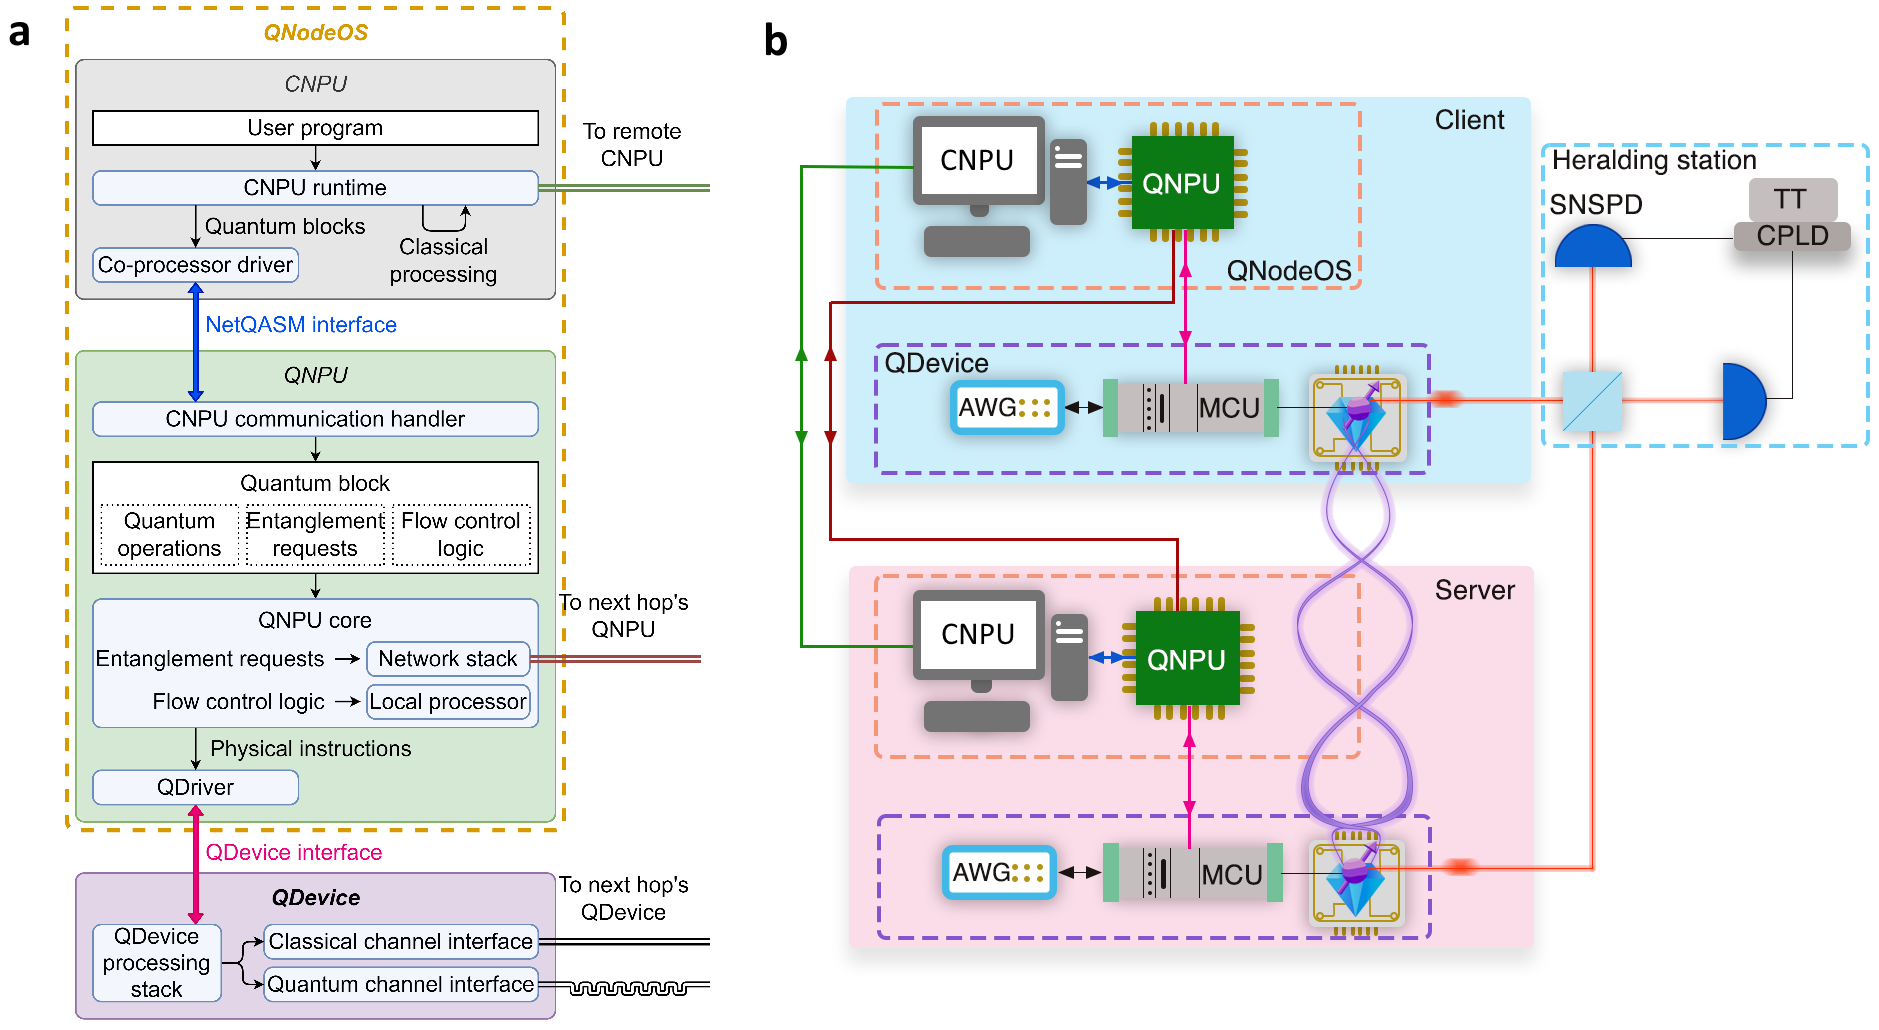
\includegraphics[width=1\linewidth]{figures/qnodeos/main/fig2/fig2.png}
\caption{\textbf{QNodeOS architecture.} \textbf{(a)} QNodeOS consists of a Classical Network Processing Unit (CNPU) and a Quantum Network Processing Unit (QNPU, classical system). QNodeOS controls a QDevice (quantum hardware and low-level classical control).
\textbf{(b)} Schematic of our implementation of QNodeOS on a two-node setup where both QDevices control a single qubit in a diamond nitrogen-vacancy (NV) center. The CNPU is implemented on a general-purpose PC, and the QNPU on an embedded system, connected via Gigabit Ethernet (blue). The QNPU connects to its QDevice via a serial peripheral interface (SPI, pink). The two QNPUs (brown), and the two CNPUS (green) connect to each other via Gigabit Ethernet. The setup is based on~\cite{pompili_2022_experimental} with two QDevices (including arbitrary waveform generators (AWG) and microcontroller units (MCU); QDevices communicating over a classical DIO interface) and a heralding station composed by a balanced 50:50 beam-splitter (whose output ports are connected to superconducting nanowire single-photon detectors (SNSPD) via optical fibers (red)),  a  TimeTagger (TT), and a \ac{CPLD} that heralds the entanglement generation between QDevices and sends a classical message to the MCU.}
\label{qnodeos:fig:fig2}
\end{figure*}

\section{Architecture}
\label{qnodeos:sec:architecture}
We divide the architecture logically into three main components (\cref{qnodeos:fig:fig2}, \cref{qnodeos:sec:methods}): The Classical Network Processing Unit (CNPU) is responsible for starting the execution of programs, and the execution of classical code blocks; the Quantum Network Processing Unit (QNPU) is responsible for governing the execution of the quantum code blocks; The CNPU and QNPU together form QNodeOS and control the QDevice, which is responsible for executing any quantum operations (gates, measurements, entanglement generation at the physical layer~\cite{dahlberg_2019_egp}) on the quantum hardware. Upon starting the execution the CNPU creates a corresponding CNPU process (a well-known concept in classical operating systems~\cite{dennis_programming_1966-1,tanenbaum_operating_2005}), registers the program on the QNPU (via the QNPU's end node application programming interface (API), \cref{qnodeos:sec:design:qnpu_stack}), which, in turn, creates its own associated QNPU process (including context such as process owner, ID, process state and priority). QNodeOS also defines kernel processes on the QNPU, which are similar to user processes, but are created when the system starts (on boot). The CNPU sends quantum blocks to the QNPU in the form of NetQASM subroutines~\cite{dahlberg_2022_netqasm}. Classical control logic in quantum blocks is executed by the QNPU processor. Quantum gates and measurements (from any QNPU process) and entanglement instructions (from the network process) are delegated to the QDevice by submitting physical instructions (\cref{qnodeos:sec:methods}), after which the QDevice responds back with the result of the instruction. 

To enable different hardware platforms, we introduce a QDriver realizing the HAL for any hardware corresponding to our minimal QDevice system model (\cref{qnodeos:sec:methods}). The QDriver is responsible for translating quantum operations, expressed in NetQASM~\cite{dahlberg_2022_netqasm}, into platform dependent (streams of) physical instructions to the underlying QDevice. We realize a QDriver for the trapped-ion system of~\cite{teller2023integrating,teller2021heating}, and one for NV centers in diamond based on the system of~\cite{hermans2022qubit,pompili_2021_multinode,pompili_2022_experimental}. We validate the trapped-ion QDriver (\cref{qnodeos:fig:fig5}) by implementing and verifying a set of single-qubit gate operations (\cref{qnodeos:sec:methods}), and the QDriver on the NV system as part of the full stack system evaluation (see below). 
To allow for different timescales, we logically divide the architecture into CNPU, QNPU and QDevice which can thus be realized at different timing scale granularities. In our proof-of-concept implementation, we realize the CNPU and QNPU on different devices, reflecting the ms timescales of communication between distant nodes (\cref{qnodeos:sec:methods}).

Ensuring the necessary interactivity requires architectural as well as implementation choices: as programs may depend on messages from remote nodes, the architecture needs to be able to dynamically handle both classical and quantum blocks, even if not known at runtime. Consequently, it is not possible to preload all quantum blocks of the program into the low-level controller of the QDevice ahead of time as done in previous physics experiments. Instead, in our system model the QDevice is capable of executing individual physical instructions similar to a classical CPU. Consequently, the QNPU is continuously ready to receive new NetQASM subroutines from the CNPU, and the QDevice can continuously receive and respond to physical instructions from the QNPU (\cref{qnodeos:sec:methods}).

In our NV QDevice implementation, we address the challenge of interactivity by interleaving specific preloaded pulse sequences (realizing physical instructions sent from QNodeOS) and dynamical decoupling (DD) sequences (protecting quantum memory from decoherence) in an arbitrary waveform generator (AWG)~\cite{zurich_instruments_hdawg_2019}. The DD sequences extend qubit coherence times up to $T_{\text{coh}} = 13(2)$ ms, while arbitrary physical instructions can be handled by triggering the corresponding pulse sequence, without knowing them in advance (\cref{qnodeos:sec:methods}).

To integrate local operations with the network schedule, our architecture first introduces a QNPU scheduler that can choose which of the ready processes is assigned to the local processor (\cref{qnodeos:fig:fig2}) and QDevice. This allows interleaving the execution of different processes directly on the QNPU without incurring delays on the timescale of the CNPU (ms), addressing the challenge of short coherence times. In our implementation, we choose to schedule QNPU processes using a priority based non-preemptive scheduler~\cite{liu_1973_scheduling}, due to limited quantum memory lifetimes, which make it undesirable to pre-empt and temporarily store quantum states while halting the execution. Second, we realize a network process as a kernel process, which manages entanglement generation using the network stack~\cite{dahlberg_2019_egp,kozlowski_2020_qnp} (implemented in~\cite{pompili_2022_experimental} without the ability to execute network applications), including a network schedule that can be determined by a time-division multiple access (TDMA) controller~\cite{skrzypczyk_2021_arch}. The network process handles entanglement requests submitted by user processes, coordinates entanglement generation with the rest of the network via the TDMA controller, interacts with the QDevice and eventually returns entangled qubits to user processes. User processes enter the waiting state when they need entanglement, and become ready again once entanglement was delivered. The network process has the highest scheduling priority, and is consequently given precedence over the execution of any local quantum operations. We remark local operations may still be executed during time-bins already occupied by the network schedule, if a running non-preemptable user process prevents the network process from running, as we indeed observe in our evaluation.

To increase utility, QNodeOS allows multiple programs to be run concurrently, using the QNPU scheduler from above to enable multitasking~\cite{mccullough_design_1965-1,dennis_segmentation_1965} user processes on the QNPU itself. The QNPU hence needs to keep context for each process, including a virtual quantum memory space (as in classical operating systems~\cite{daley_virtual_1968-1}). Similar to classical memory management systems~\cite{peterson_operating_1985}, a quantum memory management unit (QMMU) on the QNPU manages qubit allocations from processes, and translates virtual qubit addresses in NetQASM subroutines to physical addresses in the QDevice. This allows flexibility in translating a virtual qubit address to: (1) a different physical qubit address over time, allowing qubits to be rearranged transparently in the physical memory in the future, or (2) a logical qubit address, when QNodeOS is executed on top of a processor employing quantum error correction~\cite{lidar2013quantum}. Entanglement generation between different pairs of processes at remote nodes are distinguished by Entanglement Request (ER) sockets, inspired by classical sockets~\cite{chesson_network_1975-1,leach_architecture_1983}, which are established once a user process requests entanglement from the network process. In our implementation, processes of the same priority are scheduled first-come-first-served~\cite{peterson_operating_1985}, where the total schedule of the program in our implementation is dependent both on the schedule on the CNPU as well as the QNPU (\cref{qnodeos:sec:methods}).

\begin{figure*}[htbp]
\centering
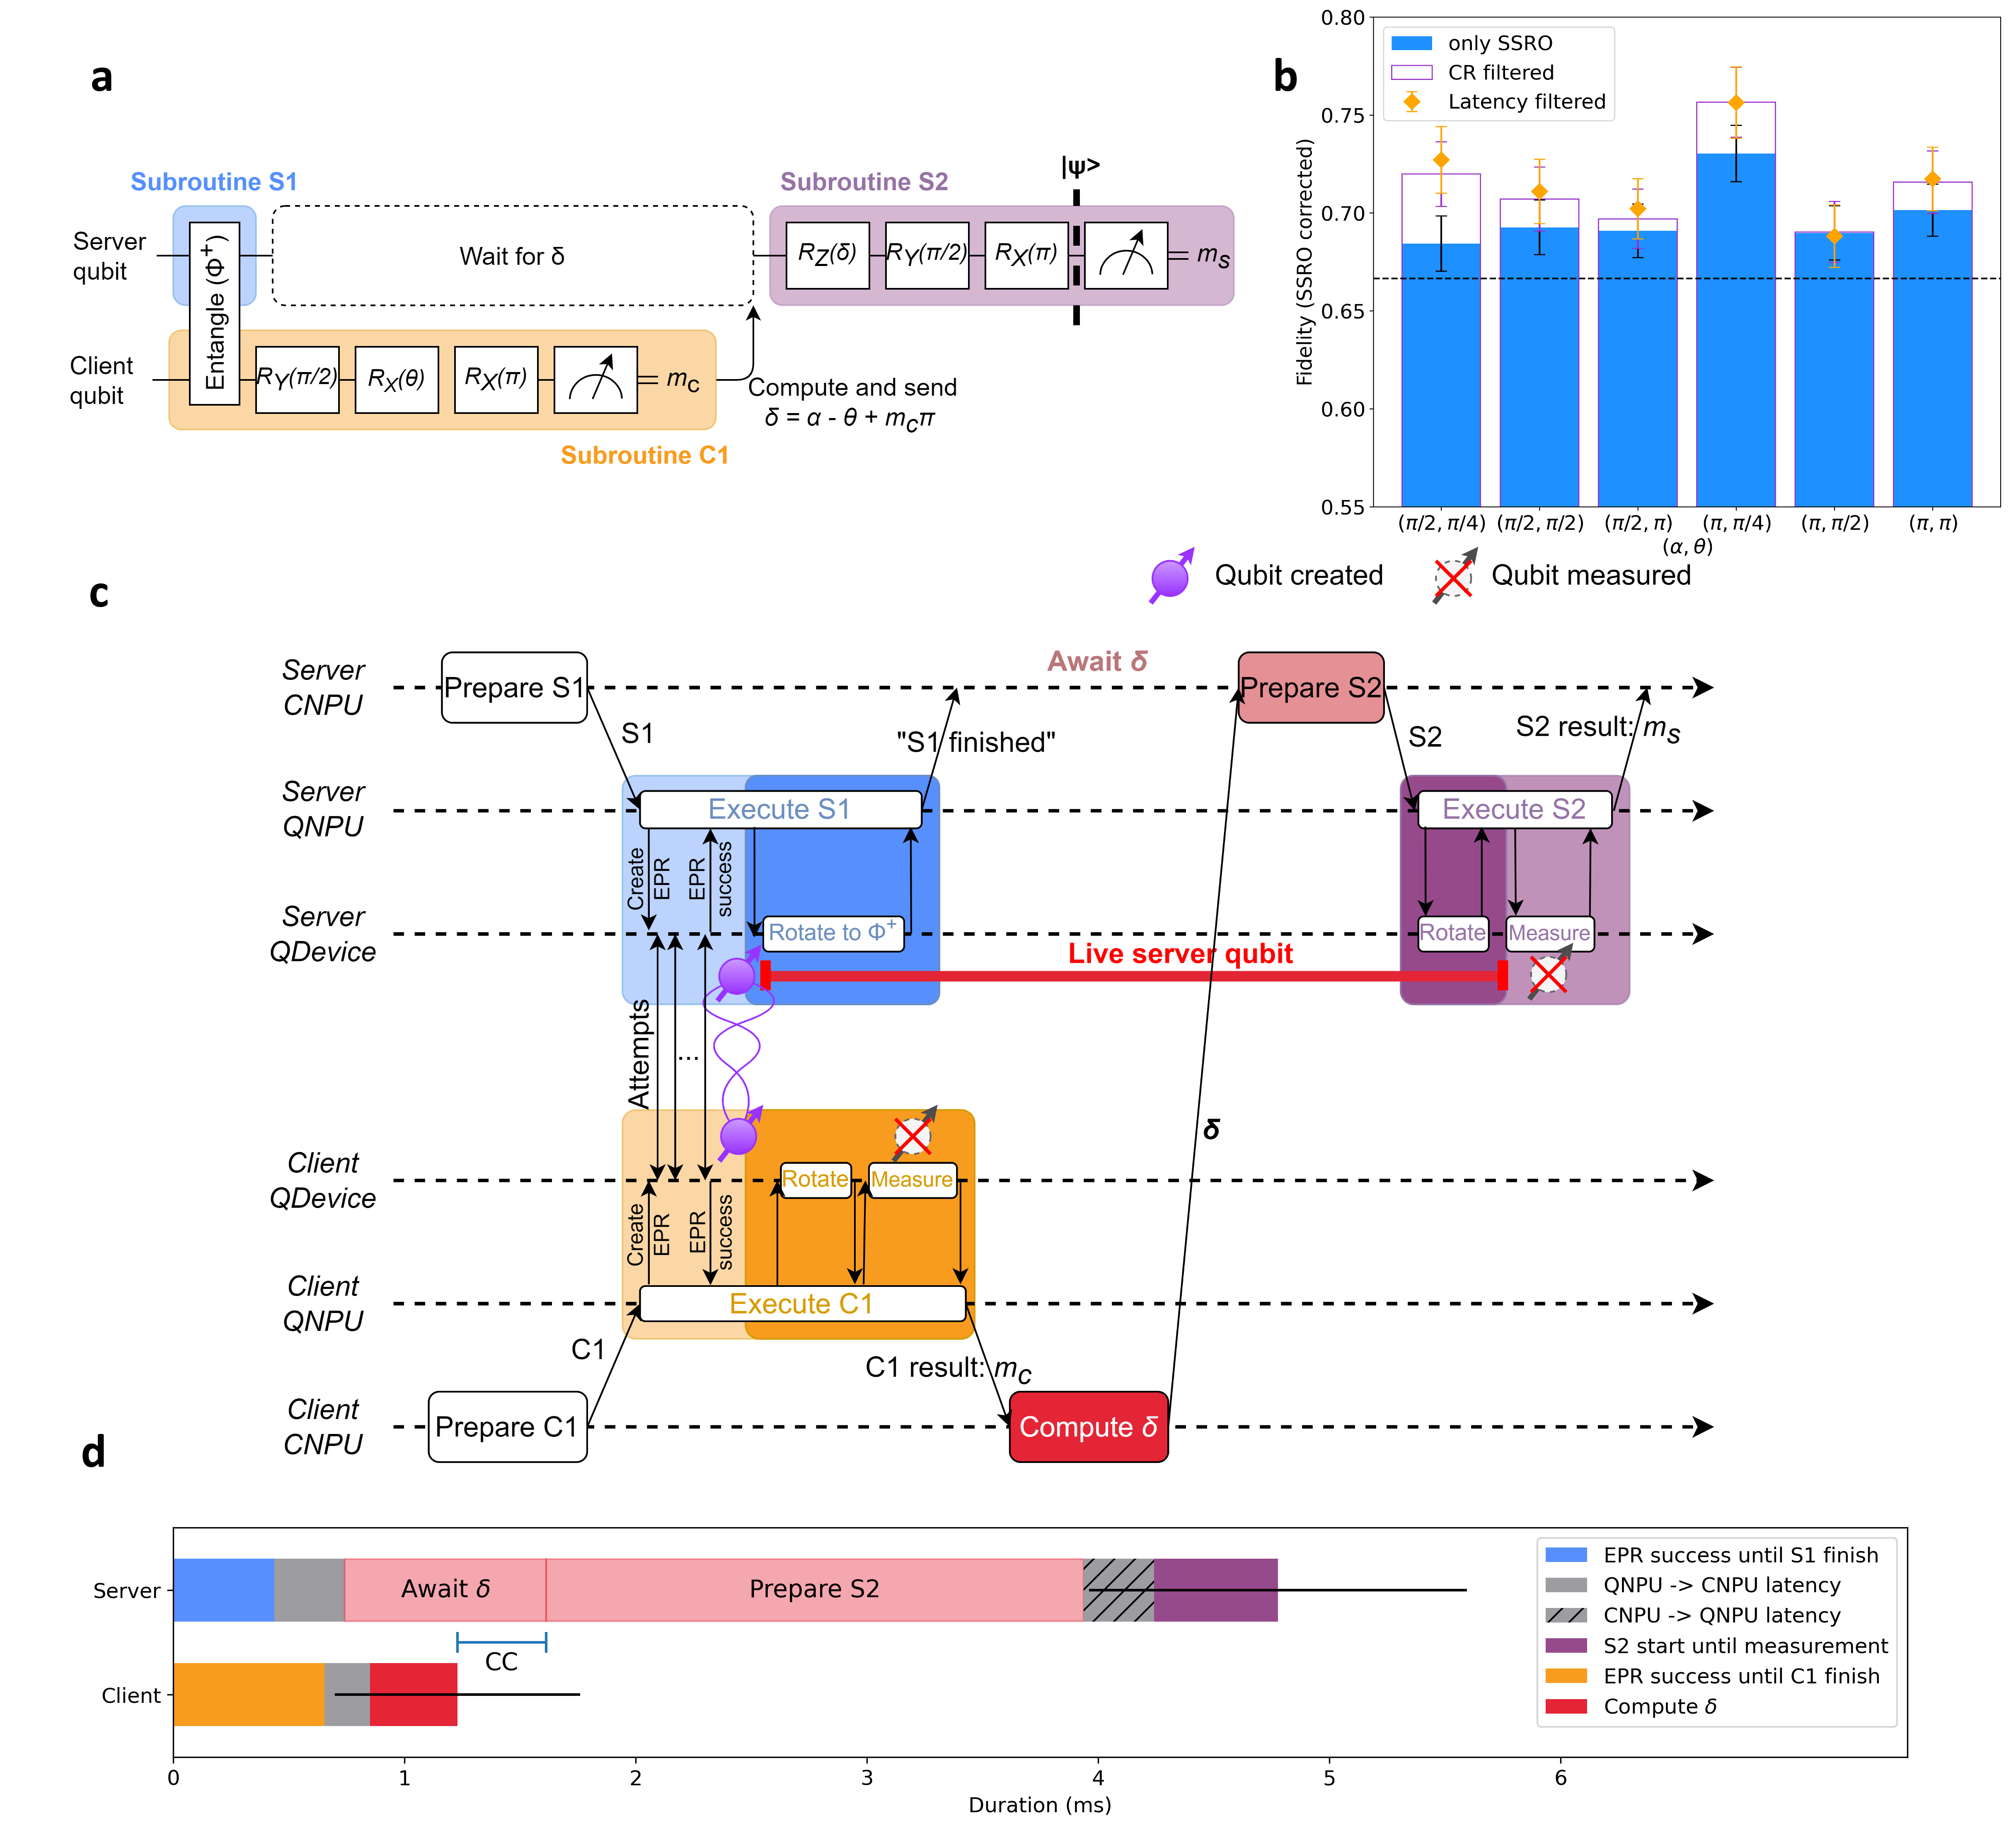
\includegraphics[width=0.89\linewidth]{figures/qnodeos/main/fig3/fig3.png}
\caption{\textbf{Delegated computation between two NV center nodes using QNodeOS.} 
\textbf{(a)} Delegated Quantum Computation (DQC) circuit (effective computation: single-qubit rotation $R_Z (\alpha)$, \cref{qnodeos:sec:methods}). The DQC application consists of $k$ repetitions of this circuit (varying measurement bases for tomography on $\ket{\psi}$) realized by two programs: the DQC-client program (client node, repeating the sequence ``quantum block (C1, orange) – classical block (computing $\delta$)'' $k$ times), and the DQC-server program (server node, repeating ``quantum block (S1, blue) - classical block (receiving $\delta$) – quantum block (S2, purple)'' $k$ times). Client and server produce an entangled pair $\ket{\Phi^+} = (\ket{00} + \ket{11}) / \sqrt{2}$ (S1 and first part of C1). The client performs local gates and a measurement (``destroying'' qubit), resulting in outcome bit $m_c$ (rest of C1). Client computes $\delta$ as function of $m_c$ and DQC parameters $\alpha \in [0,2\pi)$ and $\theta \in [0, 2\pi)$, and sends $\delta$ to server (classical message). Meanwhile the server keeps its qubit coherent (alive). Upon receiving $\delta$, the server applies gates depending on $\delta$, resulting in single-qubit state $\ket{\psi}$ (S2) depending only on $\alpha$ and $\theta$.
\textbf{(b)} Experimental results of executing DQC for 6 different sets of $(\alpha, \theta)$ parameters ($k=1200$, i.e. 7200 executions of the circuit of~\ref{qnodeos:fig:fig3}a). The fidelity of the resulting server state to the target state $\ket{\psi}$ is estimated using single-qubit tomography (1200 measurement results per data point), and corrected for known tomography errors (SSRO, blue), and post-selected for Charge-Resonance (CR) check validation (purple), and post-selected for latencies (orange) (\cref{qnodeos:sec:methods}).
\textbf{(c)} Sequence diagram including the interaction CNPU-QNPU-QDevice for one execution of the DQC circuit of \ref{qnodeos:fig:fig3}a on QNodeOS (repeated $k=1200$ times in each experiment) (time flows to the right; not to scale). CNPUs prepare NetQASM subroutines (C1, S1, S2), and send them to their respective QNPUs. CNPUs also do classical computation (computing $\delta$) and communication (message containing $\delta$). QNPUs execute subroutines, sending physical instructions to their QDevices. Entanglement is generated by QDevices doing a batch of attempts, resulting in the heralding of a two-qubit entangled state (Bell pair) rotated to $\ket{\Phi^+}$ by the server.
\textbf{(d)} Processing times and latencies while server qubit is live (time frame red line 3c, averaged over all 7200 circuit executions except executions with latency spikes, see~\cref{qnodeos:sec:methods}), including CNPU-QNPU communication latencies, CNPU processing on both nodes and client-server communication latency (CC) (average total of $\sim 4.8 (\pm 0.8)$ ms, error bars for the sum of individual segments (variance per segment in~\cref{qnodeos:sec:processing_time_latencies}).}
\label{qnodeos:fig:fig3}
\end{figure*}


\section{Demonstrations}
\paragraph{Delegated Computation}
We first validate our architecture and implementation by the first successful execution of an arbitrary – i.e. not preloaded – execution of a quantum network application in high-level software on quantum processors. We implement QNodeOS on a two-node setup of NV centers using one qubit per node (\cref{qnodeos:fig:fig2}, \cref{qnodeos:sec:methods}). We choose to execute an elementary form of delegated quantum computation (DQC)~\cite{broadbent_2009_ubqc} from a client to a server, because the client and server programs jointly realize repetitions of a circuit (\cref{qnodeos:fig:fig3}a) that triggers all parts of our system (\cref{qnodeos:fig:fig3}c). 
We first verify that the quantum result (fidelity) was found to be above the classical bound~\cite{massar_optimal_1995} $> 2/3$, which verifies that QNodeOS can successfully handle interactive applications consisting of entanglement generation, millisecond-scale memory lifetimes, and classical message passing. The non-perfect fidelity (\cref{qnodeos:fig:fig3}b) comes mainly from two sources: a noisy entangled state with fidelity 0.72(2) (quantum hardware limitation), and decoherence in the server qubit (depending on $T_{\text{coh}}$) due to waiting for several milliseconds (classical software latencies, \cref{qnodeos:fig:fig3}d).
We proceed to characterize latencies. As expected, we find that the duration that the server qubit must remain alive is dominated (> 50\%) by processing in the CNPU, which could be improved by caching the preparation of S2, and implementing the CNPU and QNPU on one board (Outlook). We observe that CNPU processing time varies significantly (standard deviation 30\%, \cref{qnodeos:sec:processing_time_latencies}), due to limited scheduling control over CNPU processes (\cref{qnodeos:sec:methods}).  Using an a priori estimate of what delays lead to too low a quality of execution (i.e. delays that are too long for the server qubit to be stored with sufficiently high quality), we discard application iterations in which the CNPU latencies spiked by more than 8.95 ms. This lead the discarding of 2\% of iterations in post-processing (\cref{qnodeos:sec:methods}).

\paragraph{Demonstration of Multitasking}
We also validate QNodeOS's multitasking capability by the first concurrent execution of two quantum applications on a quantum network: the DQC application, and a single-node local gate tomography (LGT) application on the client (\cref{qnodeos:fig:fig4}a). The two programs for the client are started in the CNPU at the same time (two CNPU processes, subject to CNPU scheduler), which means that the QNPU continuously receives subroutines for both programs from the CNPU (two QNPU processes and corresponding subroutines, subject to QNPU scheduler). This leads to a multitasking challenge directly on the QNPU to schedule the different subroutines received (\cref{qnodeos:fig:fig4}b). Since the client has only one qubit, the multitasking of DQC and LGT never results in both programs having a quantum state alive on the client; therefore, multitasking should not affect the fidelity of LGT. We observe interleaved execution of DQC quantum blocks and LGT quantum blocks on the client node (\cref{qnodeos:fig:fig4}b). The LGT application produces a quantum result (fidelity, \cref{qnodeos:fig:fig4}c) equal to that in the scenario where we run LGT on its own (not interleaved by DQC circuit executions), as expected.

We further test multitasking by scaling up the number of programs executed concurrently, up to 5 DQC and 5 LGT programs running on the client at the same time. The interleaved execution of subroutines of different programs increases device utilization (fraction of time spent on executing physical instructions) on the client QDevice compared to the same scenario but with multitasking disabled (\cref{qnodeos:fig:fig4}d). As expected, we observe that LGT subroutines were scheduled to be executed in between DQC subroutines, resulting in lower client QDevice idle time. When multitasking 1 DQC and 1 LGT program, we observe 1 or 2 subroutines in between DQC iterations in most cases (LGT subroutine duration ~2.4 ms, \cref{qnodeos:sec:multitasking-scaling}). We observe cases where both server and client QDevice remain idle, which could be improved in part by smarter CNPU-QNPU scheduling algorithms: (1) both the client and server wait until the start of the next network schedule time-bin (time-bin length 10 ms) (2) the client QNPU finishes a subroutine for user process P, but must wait until the CNPU sends the next subroutine for P (up to 150 ms for 1 DQC and 1 LGT program, but less (up to only 8 ms) when more applications are running, since there are more CNPU processes independently submitting subroutines), (3) the client is ready to perform entanglement generation for DQC, but the next time-bin starts only at some future time $t$, preventing activation of the network process. The scheduler activates a user process which runs a LGT circuit, which completes at some time $>t$, delaying the start of the DQC network process, even though the server node was ready at $t$.

\begin{figure*}[htbp]
\centering
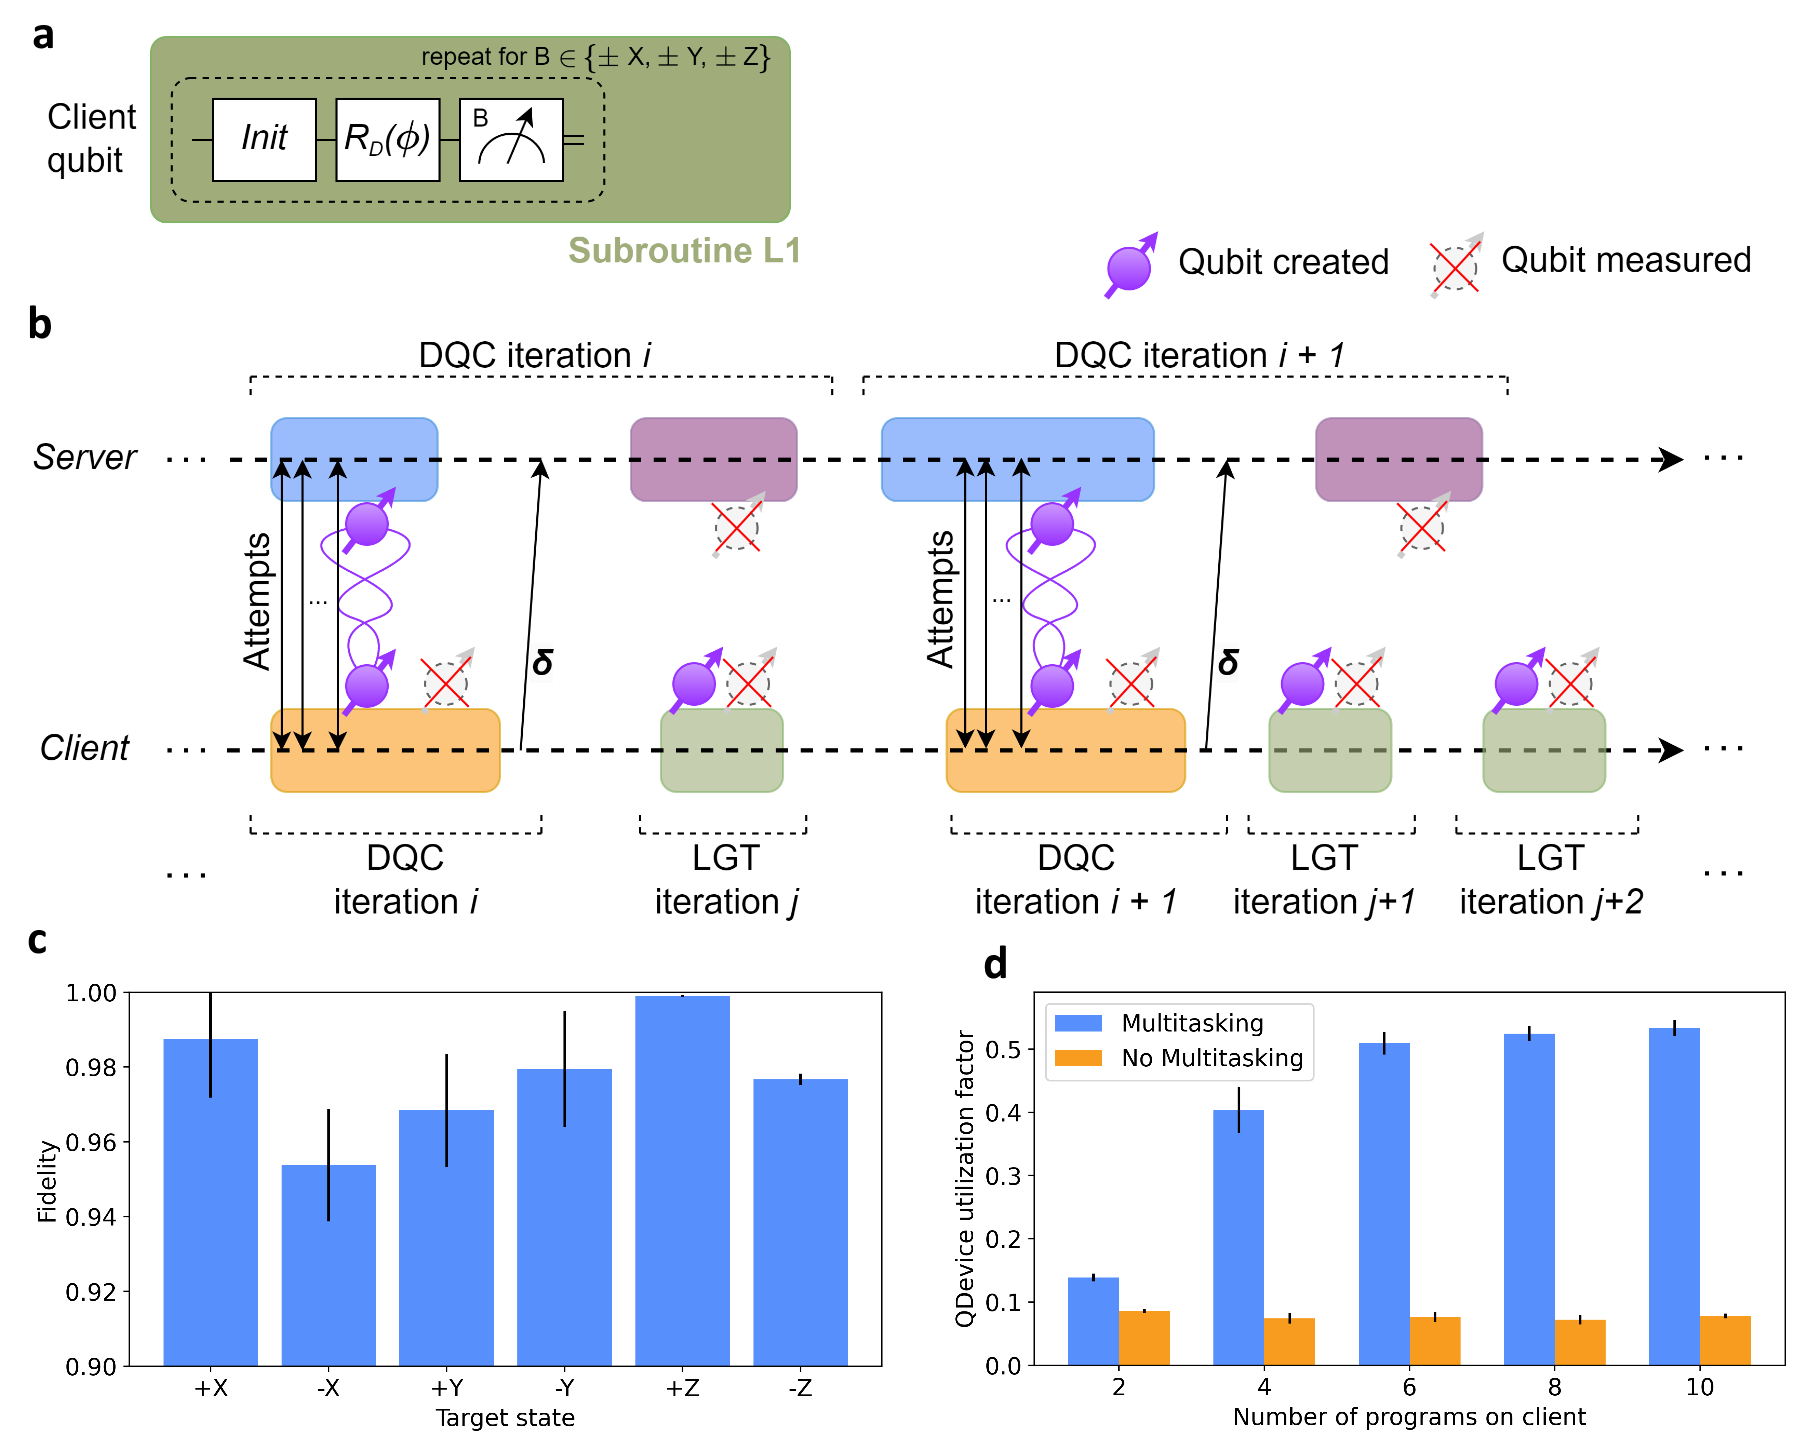
\includegraphics[width=0.95\linewidth]{figures/qnodeos/main/fig4/fig4.png}
\caption{\textbf{Multitasking experiment on two NV centers with QNodeOS}.
\textbf{(a)} Local Gate Tomography (LGT) Circuit. A single NetQASM subroutine (L1) executes the following 6 times for different bases $B \in \{\pm X, \pm Y, \pm Z\}$: initialize qubit to $\ket{0}$, rotate around fixed axis $D \in \{X,Y\}$ by angle $\ket{\phi}$, measure in $B$. The LGT application consists of a single LGT program, which submits subroutine L1 for execution to the QNPU (fixed $D$ and $\phi$) $k$ times in succession.
\textbf{(b)} Example sequence diagram illustrating concurrent execution (multitasking) of the DQC application (\cref{qnodeos:fig:fig3}) and the LGT program on the client: time slice in which two DQC circuit repetitions (\cref{qnodeos:fig:fig3}a) are realized (2 subroutines on the client (orange), 4 on the server (blue and purple)), and three LGT circuit repetitions (3 subroutines, green). The client QNPU receives subroutines for both the DQC program and the LGT program, which the QNPU scheduler can interleave: While the server executes S2 (purple), the client cannot yet execute the next S1 (orange) since it involves joint entanglement generation. In this idle time, the client can execute a number of LGT subroutines (number can vary).
\textbf{(c)} Results of multitasking LGT (client) and DQC (on both server and client). For each input pair $(D, \phi) \in \{ (X,0), (X,\pi), (Y,pi/2), (Y,-\pi/2), (X,-\pi/2), (X,\pi/2) \}$ (6 cardinal states $\{\pm X, \pm Y, \pm Z\}$), the following experiment was performed: simultaneously (1) a single LGT program was initiated on the client ($k=1000$), (2) a single DQC-client program was initiated on the client ($k=200$ successive subroutines), and (3) a single DQC-server program was initiated at the server ($k=200$, i.e. 400 successive subroutines). This resulted in a total of 6000 LGT subroutine executions and 36000 LGT measurement results, yielding plotted fidelity estimates for the LGT quantum state before measurement. Results are the same as running LGT on its own (no multitasking with DQC), as expected (\cref{qnodeos:sec:multitasking-tomography}).
\textbf{(d)} Scaling number of programs on the client. For $N \in \{1,2,3,4,5\}$, we initiate at the same time: (1) $N$ LGT programs (each using $k=100$) on the client, (2) N DQC-client programs on the client (each using $k=60$), and (3) $N$ DQC-server programs on the server (each using $k=60$). This results in $2N$ programs active at the same time on the client, each continuously submitting subroutines from the CNPU to the QNPU, where the QNPU scheduler chooses which process to execute when. Each experiment was repeated but with multitasking disabled on the client. Plot shows the utilization factor of the QDevice (fraction of time spent executing instructions), corrected for variable entanglement generation duration (\cref{qnodeos:sec:methods}), with (blue) and without (orange) multitasking, showing that multitasking can increase device utilization.}
\label{qnodeos:fig:fig4}
\end{figure*}

\section{Outlook}
We designed and implemented the first architecture allowing high-level programming and execution of quantum network applications. To deploy our system onto nodes separated by several kms it would be desirable to merge both the CNPU and the QNPU onto one system board, ideally with mutual access to a shared memory to avoid ms delays in their communication. Such a merge would also allow the definition of a joint classical-quantum executable and processes, opening further doors to reduce latencies by a better scheduling control.

Our work provides a framework for a new domain of computer science research into programming quantum network applications on quantum processors including: novel real-time~\cite{ramamritham_scheduling_1994} scheduling algorithms for classical-quantum processes, compile methods for quantum network applications, or novel programming language concepts including entanglement to make software development even easier, thus advancing the vision to make quantum network technology broadly available.


\begin{figure}[htb]
\centering
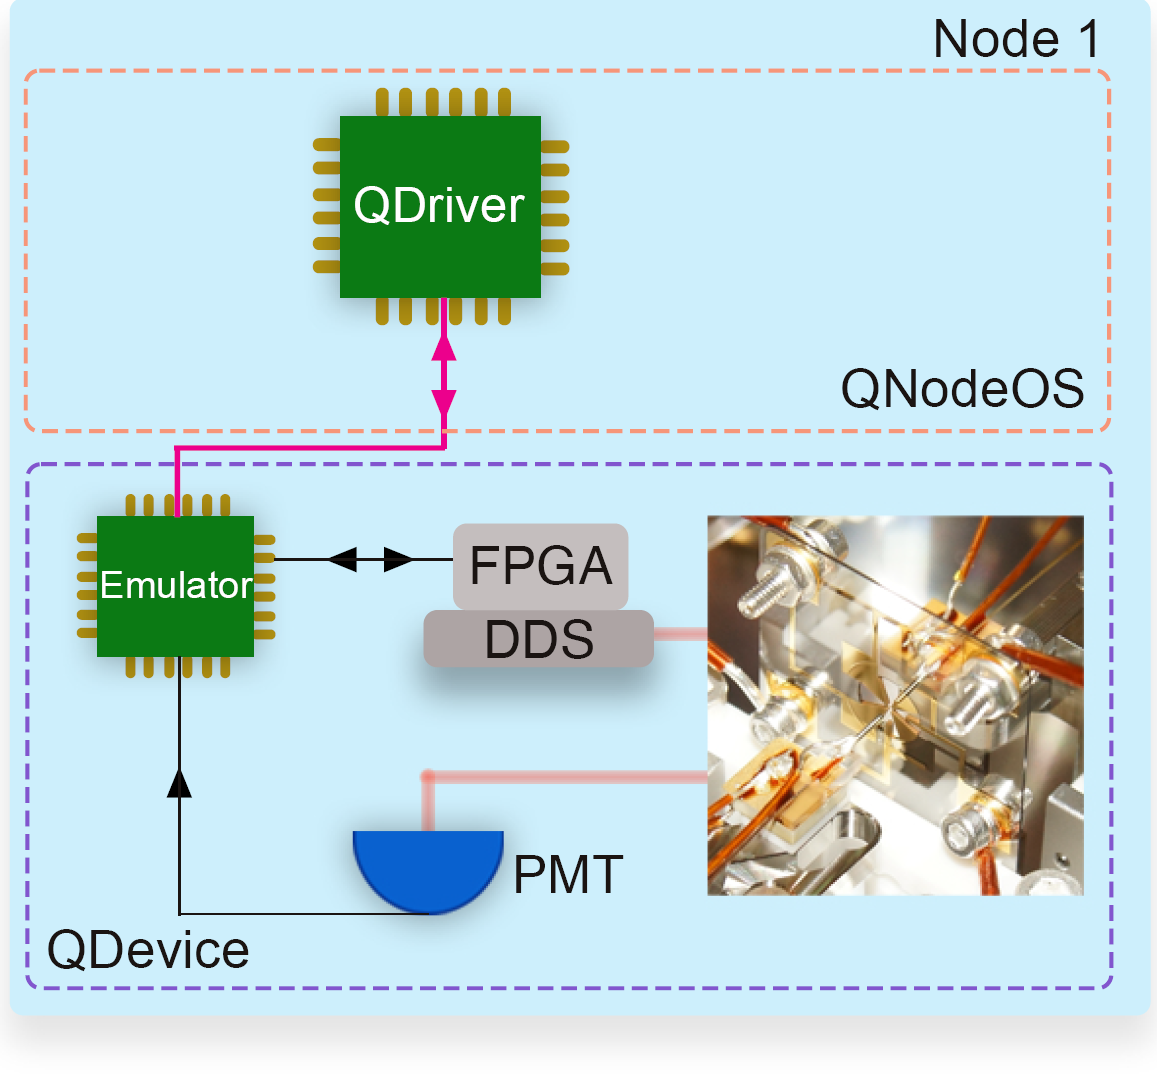
\includegraphics[width=1\linewidth]{figures/qnodeos/main/fig5/fig5.png}
\caption{\textbf{Trapped-ion QDevice implementation.} Schematic of our implementation of QNodeOS on a single-node setup in which the QDevice contains a single trapped-ion qubit. The QNPU QDriver is implemented on a field-programmable gate array (FPGA) that connects to its QDevice via a serial peripheral interface (SPI) (\cref{qnodeos:sec:methods}). The setup consists of an emulator that translates between SPI messages and TTL signals, experimental control hardware that includes an FPGA and direct digital synthesis (DDS) modules, a trapped-ion qubit~\cite{teller2023integrating} under ultra-high vacuum (\cref{qnodeos:fig:fig1}), and a photomultiplier tube (PMT) that registers atomic fluorescence.}
\label{qnodeos:fig:fig5}
\end{figure}
\section{Methods}
\label{qnodeos:sec:methods}

\paragraph{QDevice Model}

The QDevice includes a physical quantum device, which can initialize and store quantum bits (qubits) which are individually identified by a physical address, apply quantum gates, measure qubits, and create entanglement with QDevices on other nodes (either entangle-and-measure, or entangle-and-keep~\cite{dahlberg_2019_egp}). The QDevice exposes the following interface to QNodeOS (\cref{qnodeos:sec:appendix-qdevice}): number of qubits available, and the supported physical instructions that QNodeOS may send. Physical instructions include qubit initialization, single- and two-qubit gates, measurement, entanglement creation, and a `no-op' for do nothing. Each instruction has a corresponding response (including entanglement success or failure, or a measurement outcome) that the QDevice sends back to QNodeOS.

QNodeOS and the QDevice interact by passing messages back and forth on clock ticks at a fixed rate (100 kHz in our NV implementation, 50 kHz in the trapped-ion implementation). During each tick, at the same time (1) QNodeOS sends physical instruction to QDevice, (2) QDevice can send a response (for a previous instruction). Upon receiving an instruction, the QDevice performs the appropriate (sequence of) operations (e.g. a particular pulse sequence in the AWG). An instruction may take multiple ticks to complete, where the QDevice returns the response (success, fail, outcome) during the first clock tick following completion. The QDevice handles an entanglement instruction by performing (a batch of) entanglement generation attempts~\cite{pompili_2022_experimental} (synchronized by the QDevice with the neighboring node's QDevice). 

\paragraph{QNodeOS Architecture}

QNodeOS consists of two layers: CNPU and QNPU (\cref{qnodeos:fig:fig2}a, \cref{qnodeos:sec:architecture}, Supplementary). Processes on the QNPU are managed by the Process Manager, and executed by the local processor. Executing a user process means executing NetQASM~\cite{dahlberg_2022_netqasm} subroutines (quantum blocks) or that process, which involves running classical instructions (including flow control logic) on the QNPU's local processor, sending entanglement requests to the network stack, and handling local quantum operations by sending physical instructions to the QDriver (\cref{qnodeos:fig:fig2}a). Executing the network process means asking the network stack which request (if any) to handle and sending the appropriate (entanglement generation) instructions to the QDevice. 

A QNPU process can be in the following states (\cref{qnodeos:fig:process-states} in Supplementary for state diagram): idle, ready, running and waiting. A QNPU process is running when the QNPU processor is assigned to it. The network process becomes ready when a network schedule time-bin starts; it becomes waiting when it finished executing and waits for the next time-bin; it is never idle. A user process is ready when there is at least one NetQASM subroutine pending to be executed; it is idle otherwise; it goes into the waiting state when it requests entanglement from the network stack (using NetQASM entanglement instructions~\cite{dahlberg_2022_netqasm}) and is made ready again when the requested entangled qubit(s) are delivered. 

The QNPU scheduler oversees all processes (user and network) on the QNPU, and chooses which ready process is assigned to the QNPU processor. CNPU processes can run concurrently, and their execution (order) is handled by the CNPU scheduler. The QNPU scheduler operates independently and only acts on QNPU processes. CNPU processes can only communicate with their corresponding QNPU processes. Since multiple programs can run concurrently on QNodeOS, the QNPU may have multiple user processes that have subroutines waiting to be executed at the same time. This hence requires scheduling on the QNPU.

Processes allocate qubits through the Quantum Memory Management Unit (QMMU), which manages virtual qubit address spaces for each process, and translates virtual addresses to physical addresses in the QDevice. The QMMU can also transfer ownership of qubits between processes, for example from the network process (having just created an entangled qubit), to a user process that requested this entanglement. The Network Stack uses Entanglement Request (ER) sockets (opened by user programs through QNPU API once execution starts) to represent quantum connections with programs on other nodes. The Entanglement Management Unit (EMU) maintains all ER sockets and makes sure that entangled qubits are moved to the correct process.

\paragraph{NV QDevice Implementation}

The two-node network employed in this work includes the nodes “Bob” (server) and “Charlie” (client) (separated by 3 meters) described in~\cite{pompili_2021_multinode,hermans2022qubit,pompili_2022_experimental}. For the QDevice, we replicated the setup used by~\cite{pompili_2022_experimental}, which mainly consists of: an Adwin-Pro II~\cite{adwin} acting as the main orchestrator of the setup; a series of subordinate devices responsible for qubit control, including laser pulse generators, optical readout circuits and an arbitrary waveform generator (Zurich Instruments HDAWG~\cite{zurich_instruments_hdawg_2019}). The quantum physical device, based on NV centers, counts one qubit for each node. The two QDevices share a common 1 MHz clock for high-level communication and their AWGs are synchronized at sub-nanosecond level for entanglement attempts.

We address the challenge of limited memory lifetimes by employing dynamical decoupling (DD).  While waiting for further physical instructions to be issued, DD sequences are used to preserve the coherence of the electron spin qubit~\cite{de_lange_universal_2010}. DD sequences for NV-centers can prolong the coherence time ($T_{\text{coh}}$) up to hundreds of ms~\cite{hermans2022qubit} or even seconds~\cite{abobeih_2018_one_sec}. In our specific case, we measured $T_{\text{coh}}$=13(2) ms for the server node, corresponding to ~1300 DD pulses. The discrepancy to the state-of-the-art for similar setups is due to several factors. To achieve such long $T_{\text{coh}}$, a thorough investigation of the nuclear spin environment is necessary to avoid unwanted interactions during long DD sequences, resulting in an even more accurate choice of interpulse delay. Other noise sources include unwanted laser fields, the quality of microwave pulses and electrical noise along the microwave line.  

A specific challenge arises at the intersection of extending memory lifetimes using DD, and the need for interactivity: to realize individual physical instructions, many waveforms realizing are uploaded to the Arbitrary Waveform Generator (AWG), where the QDevice decodes instructions sent by QNodeOS into specific preloaded pulse sequences. This results in a waveform table, containing 170 entries. The efficiency of the waveforms is limited by the AWG's waveform granularity that corresponds to steps that are multiples of 6.66 ns, having a direct impact on the $T_{\text{coh}}$. We are able to partially overcome this limitation through the methods described in~\cite{corna_efficient_2021}. Namely, each preloaded waveform, corresponding to one single instruction, has to be uploaded 16 times in order to be executed with sample precision. To not fill up the waveform memory of the device, we apply the methods in~\cite{corna_efficient_2021} only to the DD pulses that are played while the QDevice waits for an instruction from the QNPU, whereas the instructed waveforms (gate/operation + first block of XY8 DD sequence) are padded according to the granularity, if necessary.
The physical instructions supported by our NV QDevice is given in~\cref{qnodeos:sec:qdevice-nv}.

\paragraph{NV QNPU Implementation}

The QNPUs for both nodes are implemented in C++ on top of FreeRTOS~\cite{freertos}, a real-time operating system for microcontrollers. The stack runs on a dedicated MicroZed~\cite{microzed}---an off-the-shelf platform based on the Zynq-7000 SoC, which hosts two ARM Cortex-A9 processing cores, of which only one is used, clocked at 667 MHz. The QNPU was implemented on top of FreeRTOS to avoid re-implementing standard OS primitives like threads and network communication. FreeRTOS provides basic OS abstractions like tasks, inter-task message passing, and the TCP/IP stack. The FreeRTOS kernel---like any other standard OS---cannot however directly manage the quantum resources (qubits, entanglement requests and entangled pairs), and hence its task scheduler cannot take decisions based on such resources. The QNPU scheduler adds these capabilities (\cref{qnodeos:sec:qnpu_impl_scheduler}).

The QNPU connects to peer QNPUs via TCP/IP over a Gigabit Ethernet interface (IEEE 802.3 over full-duplex Cat 5e). The communication goes via two network switches (Netgear JGS524PE, one per node). The two QNPUs are time-synchronized through their respective QDevices (granularity 10 $\mu$s), since these already are synchronized at the $\mu$s-level (common 1Mhz clock).

The QNPU interfaces with the QDevice's ADwin-Pro II through a 12.5 MHz SPI interface, used to exchange 4-byte control messages at a rate of 100 kHz.  

\paragraph{NV CNPU Implementation}

The CNPUs for both nodes are a Python runtime executing on a general-purpose desktop machine (4 Intel 3.20 GHz cores, 32 GB RAM, Ubuntu 18.04). The choice of using a high-level system was made as the communication between distant nodes would ultimately be in the ms-timescales, and this allows for ease of programming the application. The CNPU machine connects to the QNPU via TCP over a Gigabit Ethernet interface (IEEE 802.3 over full-duplex Cat 8, average ping RTT of 0.1 ms), via the same single network switch as mentioned above (one per node), and sends application registration requests and NetQASM subroutines over this interface (10 to 1000 bytes, depending on the length of the subroutine). CNPUs communicate with each other through the same two network switches.

\paragraph{Scheduler Implementation}

We use a single Linux process (Python) for executing programs on the CNPU. CNPU `processes' are realized as threads created within this single Python process. When running multiple programs concurrently, a pool of such threads is used. Scheduling of the Python process and its threads is handled by the Linux OS. Each thread establishes a TCP connection with the QNPU in order to use the QNPU API (including sending subroutines and receiving their results) and executes the classical blocks for its corresponding program. 
Both the CNPU and QNPU maintain processes for running programs. The CNPU scheduler (standard Linux scheduler, see above) schedules CNPU processes, which indirectly controls in which order subroutines from different programs arrive at the QNPU. The QNPU scheduler handles subroutines of the same process priority on a first-come-first-served (FCFS) basis, leading however to executions of QNPU processes not in the order submitted by the CNPU (\cref{qnodeos:sec:multitasking-scaling}).

Using only the CNPU scheduler is not sufficient since (1) we want to avoid millisecond delays needed to communicate scheduling instructions across CPNU and QNPU, (2) user processes need to be scheduled in conjunction with the network process (meeting the challenge of scheduling both local and network operations), which is only running on the QNPU, and (3) QNPU user processes need to be scheduled with respect to each other, (e.g. a user process is waiting after having requested entanglement, allowing another user process to be run; as observed in the multitasking demonstration). 

\paragraph{Sockets and the Network Schedule}
In an ER Socket, one node is a `creator' and the other a `receiver'. As long as an ER socket is open between the nodes, an entanglement request from only the creator suffices for the network stack to handle it in the next corresponding time-bin, i.e. the `receiver' can comply with entanglement generation even if no request has (yet) been made to its network stack.

\paragraph{Trapped-ion Implementation}

The experimental system used for the trapped-ion implementation is discussed in~\cite{teller2023integrating,teller2021heating} and is described in detail in~\cite{teller_measuring_2021}. The implementation itself is described in~\cite{fioretto_towards_2020}. We confine a single \CaPlus ion in a linear Paul trap; the trap is based on a 300 µm thick diamond wafer on which gold electrodes have been sputtered. The ion trap is integrated with an optical microcavity composed of two fiber-based mirrors, but the microcavity is not used here. The physical-layer control infrastructure consists of C++ software; Python scripts; a pulse sequencer that translates Python commands to a hardware description language for a field-programmable gate array (FPGA); and hardware that includes the FPGA, input triggers, direct digital synthesis (DDS) modules, and output logic.

QNodeOS provides physical instructions through a development FPGA board (Texas Instruments, LAUNCHXL2-RM57L75) that uses a serial peripheral interface (SPI). We programmed an additional board (Cypress, CY8CKIT-14376) that translates SPI messages into TTL signals compatible with the input triggers of our experimental hardware.
The implementation consisted of sequences composed of seven physical instructions: initialization, $R_x(\pi)$, $R_y(\pi)$, $R_x(\pi/2)$, $R_y(\pi/2)$, $R_y(-\pi/2)$, and measurement. First, we confirmed that message exchange occurred at the rate of 50 kHz as designed. Next, we confirmed that we could trigger the physical-layer hardware. Finally, we implemented seven different sequences. Each sequence was repeated $10^4$ times, which allowed us to acquire sufficient statistics to confirm that our QDriver results are consistent with operation in the absence of the higher layers of QNodeOS.

\paragraph{Metrics}

Both classical and quantum metrics are relevant in the performance evaluation: The quantum performance of our test programs is measured by the fidelity $F(\rho,\ket{\tau})$ of an experimentally obtained quantum state $\rho$ to a target state $\ket{\tau}$ where $F(\rho,\ket{\tau}) = \bra{\tau}\rho\ket{\tau}$, estimated by quantum tomography~\cite{paris_quantum_2004}. Classical performance metrics include device utilization $T_{\text{util}} = 1 - T_{\text{idle}} / T_{\text{total}}$ where $T_{\text{idle}}$ is the total time that the QDevice is not executing any physical instruction, and $T_{total}$ is the duration of the whole experiment excluding time spent on entanglement attempts (see below).

\paragraph{Experiment Procedure NV Demonstration}

Applications are written in Python using the NetQASM SDK~\cite{dahlberg_2022_netqasm} (code in~\cref{qnodeos:sec:app_source}), with a compiler targeting the NV flavour~\cite{dahlberg_2022_netqasm}, as it includes quantum instructions that can be easily mapped to the physical instructions supported by the NV QDevice. The client and server nodes independently start execution of their programs by invoking a Python script on their own CNPU, which then spawns the threads for each program. During application execution, the CNPUs have background processes running, including QDevice monitoring software.

A fixed network schedule is installed in the two QNPUs, with consecutive time-bins (all assigned to the client-server node pair) with a length of 10 ms (chosen to be equal to 1000 communication cycles between QNodeOS and QDevice as in Ref.~\cite{pompili_2022_experimental}) to assess the performance without introducing a dependence on a changing network schedule.  During execution, the CNPUs and QNPUs record events including their timestamps. After execution, corrections are applied to the results (see below) and event traces are used to compute latencies.

\paragraph{Delegated Quantum Computation}

Our demonstration of DQC (\cref{qnodeos:fig:fig3}) implements the effective single-qubit computation $\ket{\psi} = H \circ R_z(\alpha) \circ \ket{+}$ on the server, as a simple form of blind quantum computing (BQC) that hides the rotation angle $\alpha$ from the server, when executed with randomly chosen $\theta$, and not performing tomography. The remote entanglement protocol utilized is the single-photon protocol~\cite{cabrillo1999creation,bose1999proposal,hermans2023entangling} (\cref{qnodeos:sec:qdevice-nv}).

\paragraph{Filtering}

Results, with no post-selection, are presented including known errors that occur during the tomography single-shot readout (SSRO) process (\cref{qnodeos:fig:fig3}b, blue) (details on the correction Supplementary of~\cite{pompili_2021_multinode}). We also report the post-selected results in which data are filtered based on the outcome of the Charge-Resonance check~\cite{robledo2010control} after one application iteration (\cref{qnodeos:fig:fig3}b, purple). This filter enables the elimination of false events, specifically when the emitter of one of the two nodes is not in the right charge state (ionization) or the optical resonances are not correctly addressed by the laser fields after the execution of one iteration of DQC.

Additional filtering (\cref{qnodeos:fig:fig3}b latency filter) is done on those iterations that showed latency not compatible with the combination of $T_{\text{coh}}$ of the server and the average entangled state fidelity. For this filter, a simulation (using a depolarizing model, based on the measured value $T_{\text{coh}}$, \cref{qnodeos:sec:dqc-simulation}) was used to estimate the single qubit fidelity (given the entanglement fidelity measured above) as a function of the duration the server qubit stays live in memory in a single execution of the DQC circuit (\cref{qnodeos:fig:fig3}a). This gives a conservative upper bound of the duration as 8.95 ms, to obtain a fidelity of at least 0.667. All measurement results corresponding to circuit executions exceeding 8.95 ms duration were discarded (146 out of 7200 data points). 

Other main sources of infidelity, that are not considered in this analysis of the outcome, include, for instance, the non-zero probability of double excitation for the NV center~\cite{hermans2023entangling}. During entanglement generation, the NV center can be re-excited, leading to the emission of two photons that lower the heralded entanglement fidelity. The error can be corrected by discarding those events that registered, in the entanglement time-window, a photon at the heralding station (resonant Zero-Phonon Line photon) and another one locally at the node (off-resonant Phonon-Side Band photon). 

Finally, the dataset presented in~\cref{qnodeos:fig:fig3}b (not shown chronologically) was taken in “one shot” to prove the robustness of the physical layer, therefore no calibration of relevant experimental parameters was performed in between, leading to possible degradation of the overall performance of the NV-based setup.

The single qubit fidelity is calculated with the same methods as in~\cite{iuliano2024qubit}, measuring in the state $\ket{i}$ and in its orthogonal state $\ket{-i}$, provided that we expect the outcome $\ket{i}$, whereas the two-qubit state fidelity is computed taking into account only the same positive-basis correlators (XX, YY, ZZ).

\paragraph{Multitasking: Delegated Computation and Local Gate Tomography}

In the first multitasking evaluation, we concurrently execute two programs on the client: a DQC-client program (interacting with a DQC-server program on the server) and a Local Gate Tomography (LGT) program (on the client only) (\cref{qnodeos:fig:fig4}). The client CNPU runtime executes the threads executing the two different programs concurrently. The client QNPU has two active user processes, each continuously receiving new subroutines from the CNPU, which are scheduled with respect to each other and the network process.

Estimates of the fidelity (\cref{qnodeos:fig:fig4}b) include same corrections as in the Supplementary of~\cite{pompili_2021_multinode} To assess the quantum performance of the LGT application, we used a mocked entanglement generation process on the QDevices (executing entanglement actions without entanglement) to simplify the test: weak-coherent pulses on resonance with the NV transitions, that follow the regular optical path, are employed to trigger the CPLD in the entanglement heralding time-window. This results in comparable application behavior for DQC (comparable rates and latencies, \cref{qnodeos:sec:mocked_entanglement}) with respect to multitasking on QNodeOS.

\paragraph{Multitasking: QDevice Utilization when scaling number of programs}

We scale the number of programs being multitasked (\cref{qnodeos:fig:fig4}d): We observe how the client QNPU scheduler chooses the execution order of the subroutines submitted by the CNPU. DQC subroutines each have an entanglement instruction, causing the corresponding user process to go into the waiting state when executed (waiting for entanglement from the network process). The QNPU scheduler schedules another process [(56\%, 81\%, 99\%) for (N=1, N=2, N>2)] of the times that a DQC process is put into the waiting state (demonstrating that the QNPU schedules independently from the order in which the CNPU submits subroutines). The number of consecutive LGT subroutines (of any LGT process; LGT block execution time ~2.4 ms) that is executed in between DQC subroutines is 0.83 for N=1, increasing for each higher N until 1.65 for N = 5, showing that indeed idle times during DQC are partially filled by LGT blocks (\cref{qnodeos:sec:multitasking-scaling}).

Device utilization (see Metrics above) quantifies only the utilization factor in between entanglement generation time windows to fairly compare the multitasking and the non-multitasking scenario. In both scenarios, the same entanglement generation processes are performed, which hence have the same probabilistic durations in both cases. To avoid inaccurate results due to this probabilistic nature, we exclude the entanglement generation time windows in both cases.